\section{Qualitative Evaluation}

The interaction paradigm of SimpleSpeech was tested in a qualitative assessment to determine (1) the practicability of a lightweight text-based audio editor, (2) the effects of minor transcription errors on audio consumption and production, and (3) the implications of being able to edit audio in an asynchronous online discussion.

Participants were introduced to the functionality of the system, then given two untimed tasks. 
First, to simulate an asynchronous audio discussion, the test users were asked to listen to an audio comment left by the previous tester and create an original audio response. 
Next, they received a different, textual prompt and created an audio comment which would be consumed by the next user. 
In both cases the user was asked to edit his or her recording to be polished and clear.
The participants were interviewed at the end of the test; these interviews were transcribed with conversational elements filtered out.
Themes were extracted from the remaining sentences via open coding, followed by flat coding to sort statements among the themes. 
Cohen's $\kappa$ between the two coders was .78, indicating the reliability of the categorized themes.

The sample for the study consisted of 9 test subjects (4 male, 5 female, mean age 22 yrs; henceforth denoted $P_1, P_2, \ldots, P_9$). 
All participants were native English speakers. 
Two individuals, $P_2$ and $P_3$, were professional media editors who provided technical feedback and a comparison to professoinal audio editing.
The remainder were interns at edX, an educational technology non-profit, and students at RSI, a summer program for gifted high school students.

\subsection{Results}
The coding process revealed some themes that replicated the findings of Whittaker and Amento \cite{whittaker_semantic}, as well as some novel results.
For instance, the consensus was that a text-based editing paradigm provides sufficient control to render waveform manipulation unnecessary ($P_4,\,P_5,\,P_6,\,P_8$), as well as being``more accessible, more doable'' than pure waveform editing ($P_3,\,P_7$).
On the consumption side, the transcript was helpful in allowing users to ``see all the points [the speaker was] making instead of having to remember them'' ($P_3,\,P_4,\,P_6$).
Overall the presence of errors was not a heavy distractor from the content of the messages, echoing findings from Whittaker's voicemail study \cite{whittaker}, although one user described a greater focus on the audio because of these errors ($P_8$).

Although users were mostly accustomed to using the transcript for consuming the messages ($P_6$), they also pointed out that the audio gave them the ability to ``feel the emotions coming across, so ... you can still relate to what the person’s feeling'' ($P_1,\,P_5,\,P_8$).
This result indicates that text played the most significant role in \emph{factual} comprehension, while audio was most useful for \emph{tonal} comprehension.
Since both modalities seem necessary to the purpose of SimpleSpeech, we decided to maintain the combined paradigm throughout the study.

In addition to these transcript-related results, the qualitative study also yielded the following new themes:

\emph{The primary use of lightweight voice editing is to make fine-grained rather than large-scale adjustments.}
The most commonly-used manipulation during the qualitative study was the removal of disfluencies ($P_1,\,P_2,\,P_4,\,P_5,\,P_7$), followed by pause deletion ($P_2,\,P_3,\,P_5,\,P_6,\,P_8$). 
Only $P_1$ and $P_8$ edited large chunks of audio by deleting or rerecording, and $P_8$ reported doing so only to improve the smoothness of a smaller change in a sentence.
Perhaps because SimpleSpeech was presented as a tool to be briefly used to ``clean up'' recordings, participants focused on removing the ``embarrassing'' and ``awkward'' sounds ($P_1,\,P_5$). 

\emph{The linearity of audio leads to a pressure to organize one's thoughts during recording.}
$P_4,\,P_7,$ and $P_9$ described a ``psychological sort of ... need to get it all out, and the fact that it won't necessarily be as organized there.'' 
Another tester, $P_5$, had ``a tendency to get like a blank slate'' in which he ``couldn't think of anything to say.'' 
The elevated mental task load that $P_5$ describes could be inherent in oral discussion; $P_9$ noted that ``[it] might just be the fact that I was recording,'' and that ``editing would make it nicer.'' 
Users likely reported this pressure despite the capability to edit their recordings due to the previous theme of lightweight editing, and also because this pressure arose in the moment of recording rather than throughout the entire message-composition workflow.

\emph{Awareness of the recipient and the editability of the audio drive up the quality of contributions.}
Four users mentioned the formality of their recordings ($P_1,\,P_5,\,P_7,\,P_9$), which they attributed to ``an expectation'' to edit, given that ``someone else would know that I had that opportunity'' ($P_8$).
As $P_9$ explained her motivation to edit:
\begin{quote}
	Personally I'm editing to express myself a little more in a polished way when I'm writing.... especially if I know someone else is going to review it and be able to respond, I want to make sure I'm as clear as possible and as concise in a way that doesn't really come across when I'm talking.
\end{quote}
Listening to another participant before initiating their own comment may have been a factor in determining the users' performance ($P_9$), as well as the presence of editing tools: ``Since you have the ability to edit things, it feels like you're talking to somebody who's prepared a point or a conversational view'' ($P_5$). 
The negative viewpoints of a few users on the editing ability were generally expressed in similar terms, so we considered this theme important for the success of AAC.

\section{Quantitative Evaluation}
Our second, quantitative experiment was conducted in order to validate the three original themes identified in the qualitative evaluation above.
In doing so, these measurements collectively assess the efficacy of SimpleSpeech and, indirectly, the usefulness of audio editing tools in general for educational discussions.

\subsection{Procedure}
Two between-subject dimensions were studied: students versus teachers, as well as the formality of initial stimulus recordings (see ``\nameref{stimuli}'' below).
In addition, the dimension of no-editing versus editing was studied on a within-subject basis.
Participants in the study were given two task parts in random order: recording messages without editing functionality (the \textbf{No Editing}, or \textbf{NE} task) and using SimpleSpeech (the \textbf{Editing}, or \textbf{E} task). 
Each task consisted of ``discussion threads,'' in which users read a prompt statement, listened to another person's opinion on the issue, then produced an original response.
Participants responded to two threads for each task, for a total of four messages of about one-minute duration each.
(Before starting the E part, participants were given a standardized tutorial to learn how to edit using SimpleSpeech.)

After each task, the NASA Task Load Index (NASA-TLX) questionnaire was used to quantify the pressure or mental task load of producing a voice message \cite{nasatlx}. 
NASA-TLX is a subjective analytical tool that measures task load along six dimensions: Mental Demand, Physical Demand, Temporal Demand, Performance, Effort, and Frustration. 
Participants in the study completed the TLX ranking and weighting procedure after each task to obtain comparisons between the no-editing and editing situations.

The quantitative study was conducted at a small suburban public high school in the midwestern U.S. with 28 volunteer participants (16 students, ages 16-18, and 12 teachers; 13 male, 15 female).
This location was ideal for the study because the sample contained a variety of learning and speaking styles as well as different aptitudes for technology and discussion. 

\subsubsection{Stimuli and Formality Measures}\label{stimuli}
The criterion used for formality was the F-score, a measure of contextuality introduced by Heylighen and Dewaele in 2002 \cite{heylighen}.
The F-score is a purely textual metric based on the frequencies of various parts of speech in a text: nouns, adjectives and prepositions decrease contextuality and increase the F-score since they are independent of the circumstances around the text, while verbs, adverbs, pronouns, and interjections increase contextuality and decrease the F-score. 

The initial stimulus recordings for each of the prompt statements were generated by a group of five initial volunteers, who were asked to plan and edit some of the comments and improvise on the others. 
After splitting the resulting messages by formality, the average F-score was 53.7 for the Group A messages and 49.4 for the Group B messages ($p=.11$ by unpaired $t$-test), reflecting the likely greater contextuality of the recordings produced on-the-fly.
Group A stimuli also tended to use longer words than those for Group B (4.62 versus 4.38 letters, $p=.047$), to be more concise (113 versus 193 words, $p=.0095$), and to have higher speaking rates (149 compared to 134 words per minute, $p=.076$).
After obtaining and categorizing these messages, the voices were anonymized by adjusting the pitch randomly.

Since the qualitative study had indicated that prior exposure to other individuals' messages could affect the perceived formality in the discussion, half the participants (Group A) listened to only formal recordings, while the other half (Group B) listened to only informal ones.
We hypothesized that the participants in Group A would produce more formal messages due to the stimuli they received.

\subsection{Results}
We analyzed the effects of the live voice editing features by analyzing system logs, speech contents, and the task load survey data. The results fell into the following three categories:

\begin{table*}
	\centering
	\begin{tabular}{r c c c c}
		& \multicolumn{2}{c}{\textbf{Students}} & \multicolumn{2}{c}{\textbf{Teachers}}\\
		& \multicolumn{2}{c}{$(N=16)$} & \multicolumn{2}{c}{$(N=12)$}\\
		\toprule
		Task			& \textit{E} & \textit{NE} & \textit{E} & \textit{NE}\\
		Mental Demand   & 9.56 (1.0) & 11.1 (1.0) & 11.4 (1.3) & 10.8 (1.4) \\
		Physical Demand & 3.69 (0.6) & 2.63 (0.5) & 4.00 (1.3) & 2.83 (0.6) \\
		Temporal Demand & 7.81 (1.1) & 10.5* (1.0) & 7.50 (1.4) & 10.0 (1.3) \\
		Performance     & 8.25 (0.7) & $10.0^+$ (0.6) & 8.50 (1.4) & 9.67 (1.3) \\
		Effort          & 9.06 (1.1) & 11.6* (0.9) & 9.83 (1.7) & 10.4 (1.4) \\
		Frustration     & 7.75 (1.1) & 8.88 (1.0) & 8.42 (1.6) & 10.0 (1.7) \\
		\midrule
		Total (weighted)& 8.70 (0.7) & 10.8* (0.6) & 9.47 (1.2) & 10.6 (1.3) \\
		%& \multicolumn{2}{c}{$p=.011$} \\
		\bottomrule \\
	\end{tabular}
	\caption{The unweighted mental work load ratings reported by students and teachers from recording voice messages. \textit{E} and \textit{NE} refer to the tasks in which editing was allowed and disallowed, respectively. Each value ranges from 1 to 20, indicating the subjective level of task load that participants rated for each metric; standard error is given in parentheses. ($^+$ -- $p<0.10$, * -- $p<0.05$, paired two-tailed comparison of \textit{E} and \textit{NE})}~\label{tab:table1}
\end{table*}

\subsubsection{Utilization of SimpleSpeech Features}
As in the qualitative study, most participants appreciated and took advantage of the ability to edit their messages. They found the interface intuitive and natural, presumably due to familiarity with text-editing interfaces. 

The amount of editing that users engaged in varied widely: on average, about 17.7 edits were made to each comment (\textit{SE} = 2.3, including inserting a new recording, inserting a pause, deleting words, or deleting a pause). 
Of these changes, the vast majority were subtractive: 6.6 word deletions (\textit{SE} = 1.6) and 6.3 pause deletions (\textit{SE} = 1.1) per message.
This was consistent with the previously-observed inclination to remove disfluencies and ``awkward'' hesitations from the recordings.
Both teachers and students exhibited this impetus with no significant difference (12 deletions for students, 16.2 for teachers, $p=.36$ by unpaired $t$-test), so correcting misspeeches was fairly universal across participants.
Insertions of any kind were less common, at 1.1 per message (\textit{SE} = 0.3), probably because users tended to correct themselves \emph{post hoc} during the initial take and delete the mistakes afterward.
Four users went without performing any edits at all on at least one message; three out of these were teachers, and their messages were generally already fluent.

One error that several participants made was to use the Delete key on tokens to fix transcription errors, which resulted in the permanent deletion of that audio token. 
However, emphasis in the tutorial that the Delete key deleted the audio permanently did help other participants avoid making this mistake.
Another misconception we observed in a few participants was a tendency to treat SimpleSpeech as a dictation tool. 
These users paused for long periods of time during recording sessions and neglected to play back the messages during editing. 
Furthermore, their inclination after stopping a recording session was to go back and correct transcription errors so that the visual representation made sense.

\subsubsection{Effect on Task Load}
Since the NASA-TLX scale is subjective, it does introduce variability between participants due to the differences between their perceived skill at the task \cite{nasatlx}. 
For instance, one participant could rate the recording task at a 3 out of 20, while another could rate the very same task at a 15.
Therefore, the strongest comparisons of task load were made in the within-subject dimension, which was the ability or inability to edit.

Overall, the students reported significantly \emph{lower} levels of mental task load or pressure during the E task than the NE task (8.70 compared to 10.8, $p=.011$ by paired $t$-test). 
The values for the individual components of the TLX, shown in Table \ref{tab:table1}, yielded the following contributory dimensions on the TLX questionnaire:

\begin{itemize}
	\item \emph{Temporal demand}. Students rated the temporal demand at 7.81 for the E task, significantly less than the NE rating of 10.5 ($p=.037$ by paired $t$-test). 
	As described by the TLX form, temporal demand refers to ``time pressure due to the rate or pace at which the tasks or task elements occurred'' \cite{nasatlx}.
	Students verbally described the increase in time demand reported on the TLX in terms of having to think of words quickly, with the knowledge that every second not filled with speech would be an embarrassing silence.
	\item \emph{Performance}. Students felt more concern about the quality of their messages in the NE task, with a marginally significant difference of 10.0 compared to 8.25 for the E task ($p=.083$ by paired $t$-test). 
	Just as the participants in the prior qualitative study had articulated a desire to make their messages better for the sake of their listeners, the students also evidently wanted to improve their recordings in the NE task. 
	The inability to do so resulted in elevated task load due to performance, while for the E task the stress was lower because they were afforded the chance to correct their mistakes.
	\item \emph{Effort}. Similarly to performance, students reported having to work significantly harder in the NE task to complete it to their desired level (rated 11.6 compared to 9.06 in the E task, $p=.014$ by paired $t$-test). 
	This increased effort could correspond to the additional mental activity which had to be expended in order to generate speech fluently and without excessive hesitation.
\end{itemize}

While the teachers also reported slightly lower average workload levels in the E task, as shown at the right of Table \ref{tab:table1}, this difference was not significant.
In fact, 7 of the 12 participating teachers actually rated the E task as requiring a higher workload than the NE task.
This subset of the teachers, 5 of whom were in Group A, reported an average task load greater in the E task than the NE task for \emph{all} dimensions.
The reason for this rating, these teachers explained, was that the availability of the editing tools caused them to feel more worried about their performance (likely due to $P_8$'s ``expectation to edit'').
They were thus made to expend more effort to preserve the existing fluidity of their messages.

Overall, the fact that the differences in perception of workload varied so much among teachers indicates that they were not as heavily affected by the ability to edit as the students, who clearly appreciated the security that SimpleSpeech offered.

\subsubsection{Speech Formality Between Subject Groups}
\begin{table*}
	\centering
	\begin{tabular}{r c c c c}
		\toprule
		& \multicolumn{2}{c}{\textbf{Students}} & \multicolumn{2}{c}{\textbf{Teachers}} \\
		Group                        & \textit{A} & \textit{B}  & \textit{A} & \textit{B} \\
		Formality (F-score)          & 55.8 (1.1)   & 53.4 (1.3)         & 54.7 (1.6)   & 55.5 (1.5)\\
		Word length                  & 4.40 (0.06)   & 4.44 (0.05)           & 4.50 (0.06)    & 4.47 (0.06)\\
		Disfluencies (per 100 words) & 1.59 (0.35)    & 2.38 (0.41)          & 1.27 (0.27)    & 1.41 (0.38)\\
		Word count                   & 101 (6.5)  & $140^+$ (13)      & 155 (19)  & 130 (9.4)\\
		Speaking rate (words/min)    & 130 (5.0)  & 115* (3.8)      & 137 (6.8)  & 138 (4.9)\\
		\bottomrule \\
	\end{tabular}
	\caption{Various metrics describing the formality of the audio messages produced by each participant group. Group A listened to more formal initial stimulus recordings than Group B. There were few significant differences in these criteria between the groups, indicating that formality was dependent on the general context of AAC as well as the speaker's preference, especially for teachers. Standard error is given in parentheses. ($^+$ -- $p<0.10$, * -- $p<0.05$, unpaired two-tailed comparison of groups A and B)}~\label{tab:formality}
\end{table*}

Contrary to the hypothesis that prior exposure to audio messages would affect the formality or linguistic traits of new messages, the F-scores of the participants' output were unrelated to the group they were in, as shown in Table \ref{tab:formality}.
However, the students' speaking rates in Group A were significantly faster than those in Group B ($p=.016$ by unpaired $t$-test).
Moreover, students in Group B spoke significantly \textit{slower} than teachers exposed to the same stimulus recordings ($p=.0016$ by unpaired $t$-test), but there was no corresponding difference in Group A.
This may reflect the auditory component of formality observed by the qualitative test users, if the faster speaking rate was interpreted by students as thought-out or engaging speech.

Interestingly, the same teachers who reported higher task load in the editing task also produced more formal messages than the other teachers (mean F-score 56.6 compared to 53.0, $p=.12$ by unpaired $t$-test) and with longer words (4.58 compared to 4.35 letters, $p=.0082$).
In fact, the student participant group also contained members who rated the E task as more demanding than the NE task, though fewer in number (4 out of 16); these students produced much more formal messages than their peers as well (F-score 57.9 compared to 53.5, $p=.027$ by unpaired $t$-test). 
These participants could have had more experience speaking extemporaneously or felt less inclined to speak conversationally, ultimately leading to SimpleSpeech not being as useful to them.

On the whole, the formality of the recordings was not affected by the stimulus message or even whether the participant was a teacher or a student.
Considering that the F-score measures contextuality between the speaker and the audience, the principal sources of variation in F-score must have been personal aptitude and preference for the medium and the scenario of an online forum discussion.

\section{Formality Comparison}
Contextuality in the online voice-based discussion scenario could be highly indicative of AAC's potential applications, and to our knowledge this trait has not been studied extensively.
We therefore conducted a comparison between the voice messages composed during this study and several publicly-available corpora.
To our knowledge, no corpus exists that was collected in an audio-text situation like SimpleSpeech, so contrasts in formality inevitably arise from the differences in medium. 

The SimpleSpeech text, representing AAC, contained 14,569 words from 112 messages.
For written documents, we used several sections of the well-known Brown corpus to compile general categories of text: nonfiction, fiction, and technical writing (consisting of government documents, scientific articles, and news) \cite{brown}.
We obtained chatroom text from the \texttt{nps\_chat} corpus, face-to-face conversation data from the \texttt{webtext} corpus, and telephone data from the \texttt{switchboard} corpus, all available as part of the Natural Language Toolkit (NLTK) \cite{nltk}.
Finally, we also analyzed email communication in non-spam messages from the Enron corpus \cite{enronsent}, as well as a corpus of Twitter posts \cite{twitter}.

The results of this comparison, shown in Fig. \ref{fig:formality}, illustrate the middle-ground that AAC takes relative to oral and written media. 
The least formal and most contextual corpora were those based on oral communication (with the notable exception of web chat messages), while the most formal and least context-dependent were the written texts, including email and Twitter posts. 
We will note three possible explanations for the formality of each medium based on the ordering of the corpora:

\begin{figure}
	\centering
	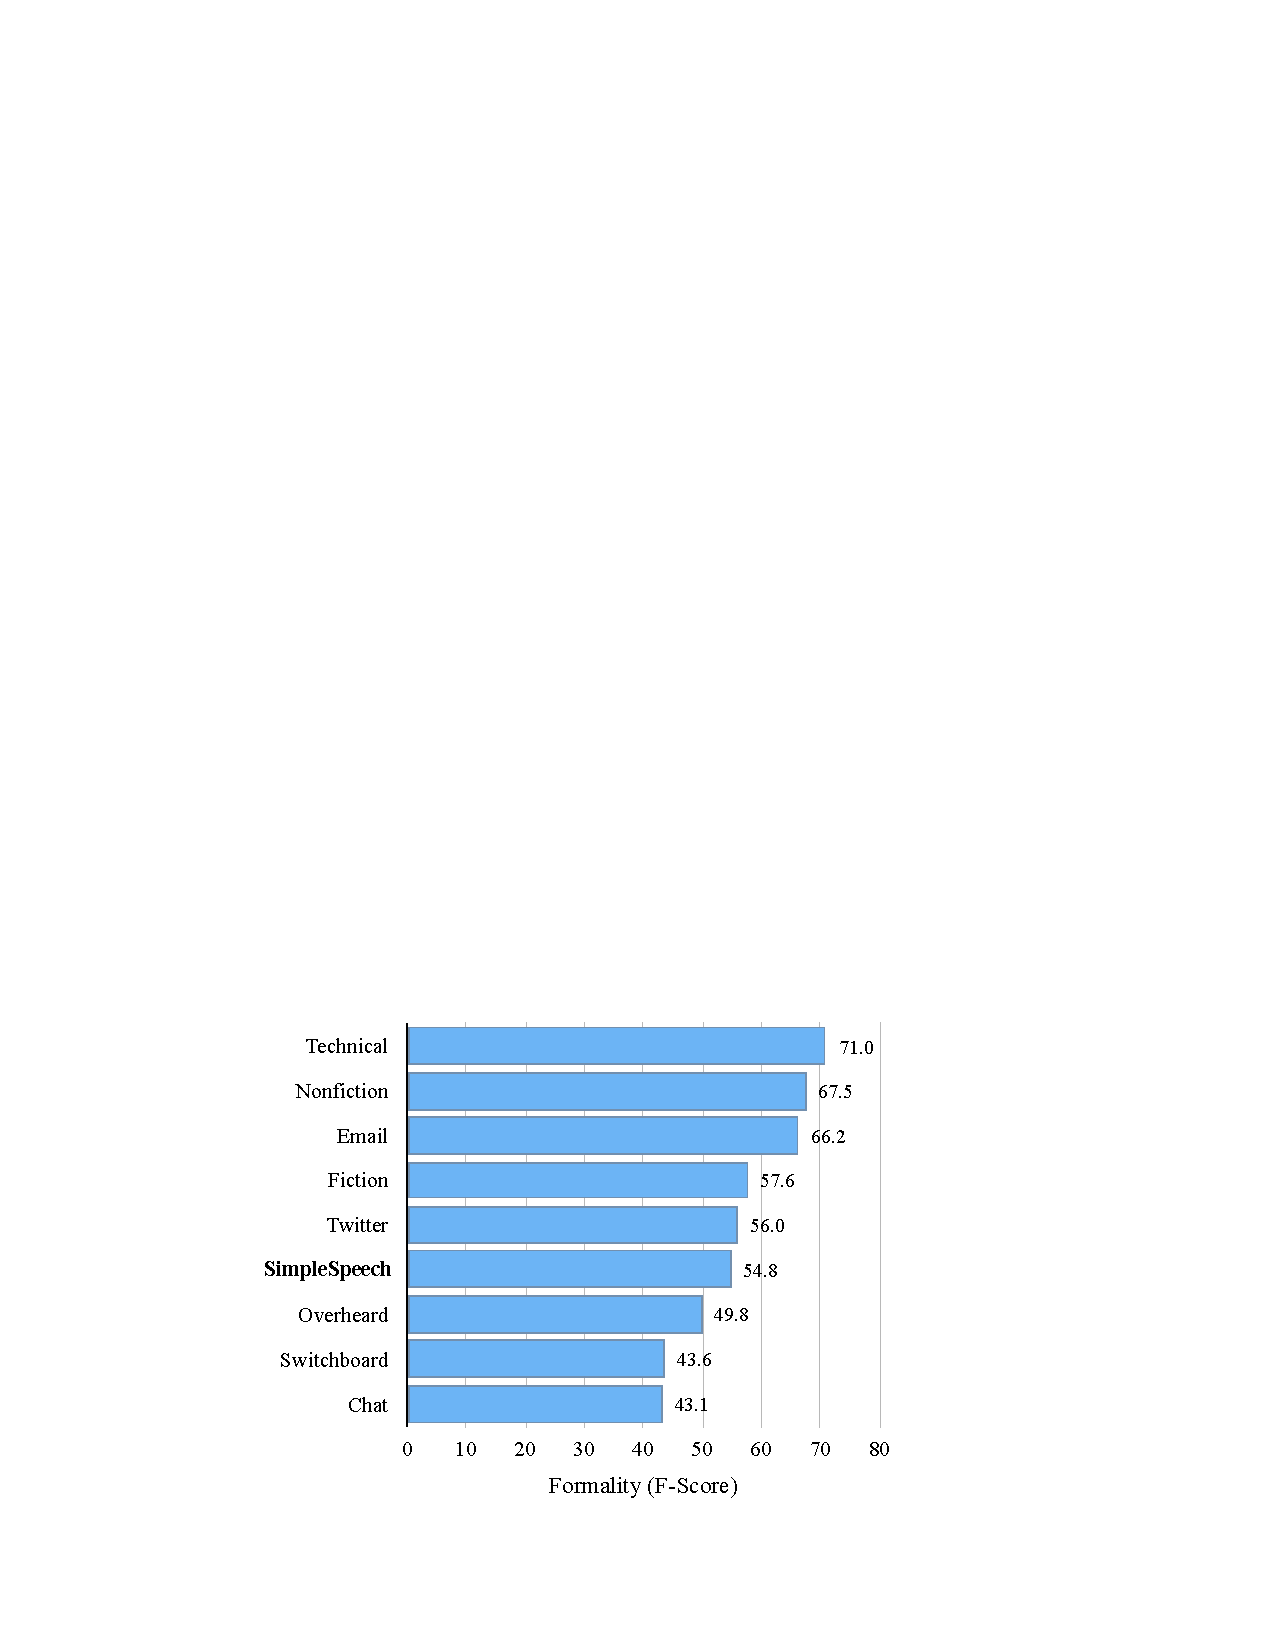
\includegraphics[width=\columnwidth,keepaspectratio]{figures/formality_comparison}
	\caption{The formality of corpora in different genre and media. The messages produced using SimpleSpeech during the quantitative study are intended to reflect general AAC discussion characteristics, and seem to be more formal than other spoken forms of communication but not as formal as email.}~\label{fig:formality}
\end{figure}

\emph{Speaker-audience relationship}. 
Since the F-score is inversely related to contextuality, it is reasonable that the chat and telephone corpora had the lowest F-scores because the participants knew each other and were conversing on a one-to-one basis. 
On the other hand, the written forms of communication (with the exception of email) were more formal because the audience was defined more loosely and not necessarily acquainted with the speaker.
AAC using SimpleSpeech was more closely related to the latter condition (as an online forum discussion), which probably contributed to its greater formality compared to the other spoken corpora.

\emph{Immediacy of communication}. 
The tendency to speak or write more contextually when the recipient must respond immediately helps explain why the online chat text, though written, was more contextual and less formal than the oral corpora. 
It also justifies the fact that the email corpus was more formal than all of the other direct communication media.
Again, AAC falls toward the more formal end of this spectrum because there is little temporal proximity between the speaker and the audience.

\emph{Tendency toward verbosity}.
Media that pressured the creator to be brief or precise were more formal and less contextual.
For instance, writing technical documents requires the preferential use of nouns over pronouns to maximize clarity.
Twitter messages are, of course, limited to 140 characters, leading to a greater concentration of meaning that favors less contextual words.
For AAC, the ability to edit could potentially influence the contextuality if discussion members were pressured to trim down their recordings. 
For our study, however, the F-score was not affected by verbosity, because edits were more concentrated on removing disfluencies and misspeeches than on improving concision.
